Sikteeri on vuosien varrella paisunut yleiseksi toiminnanohjausjärjestelmäksi, jonka arkkitehtuuria kehittäjät haluaisivat viedä palvelusuuntautuneiden arkkitehtuurien suuntaan, jotta yksittäisten palveluiden kehittäminen olisi kevyempää. Eräs suunnitteilla oleva palvelu on käyttäjien palvelunhallinta, jota kautta jäsenet voisivat lisätä itselleen jäsenmaksuun kuuluvia palveluita, kuten sähköpostialiaksia ja domaineja. Jäsenet kirjautuvat palveluhallintaan henkilökohtaisella Kapsi ry:n käyttäjätunnuksella. Jotta Sikteerin ulkopuolisten web-palveluiden kehittäminen on mahdollista, täytyy erillisillä palveluilla olla tapa tunnistaa käyttäjä.

Varsinainen käyttäjähallinta on tällä hetkellä Sikteerin ulkopuolisessa LDAP-tie\-to\-kan\-nas\-sa. LDAP-tietokannan data synkronoidaan Sikteerin omaan tietokantaan, johon tallennettujen tunnistetietojen perusteella Sikteeri tunnistaa käyttäjät. Tulevaisuudessa tietojen synkronointia ei haluta tehdä, vaan käyttäjien tunnistetiedot halutaan säilyttää vain LDAP-tietokannassa. Koska käyttäjätietokantaan on tallennettu henkilökohtaista dataa, kuten henkilötunnuksia, halutaan integroinnit siihen pitää mahdollisimman vähälukuisina.

Tällä hetkellä käyttäjien tunnistamista vaativia sovelluksia on vain Sikteeri ja admtool, mutta pidemmän aikavälin tavoitteena on uusien palveluiden (kuten käyttäjien palvelunhallinta) toteuttaminen. Nykyisiä ja tulevia palveluita varten halutaan toteuttaa keskitetty tunnistautumispalvelu, jolla on pääsy LDAP-tietokantaan ja joka tunnistaa käyttäjät. Kuvassa \ref{kapsi_nykyinen_uusi} on nykyisten hallintatyökalujen arkkitehtuuri, kun kuvaan on lisätty keskitetty tunnistautumispalvelu.

\begin{figure}[ht]
\centering
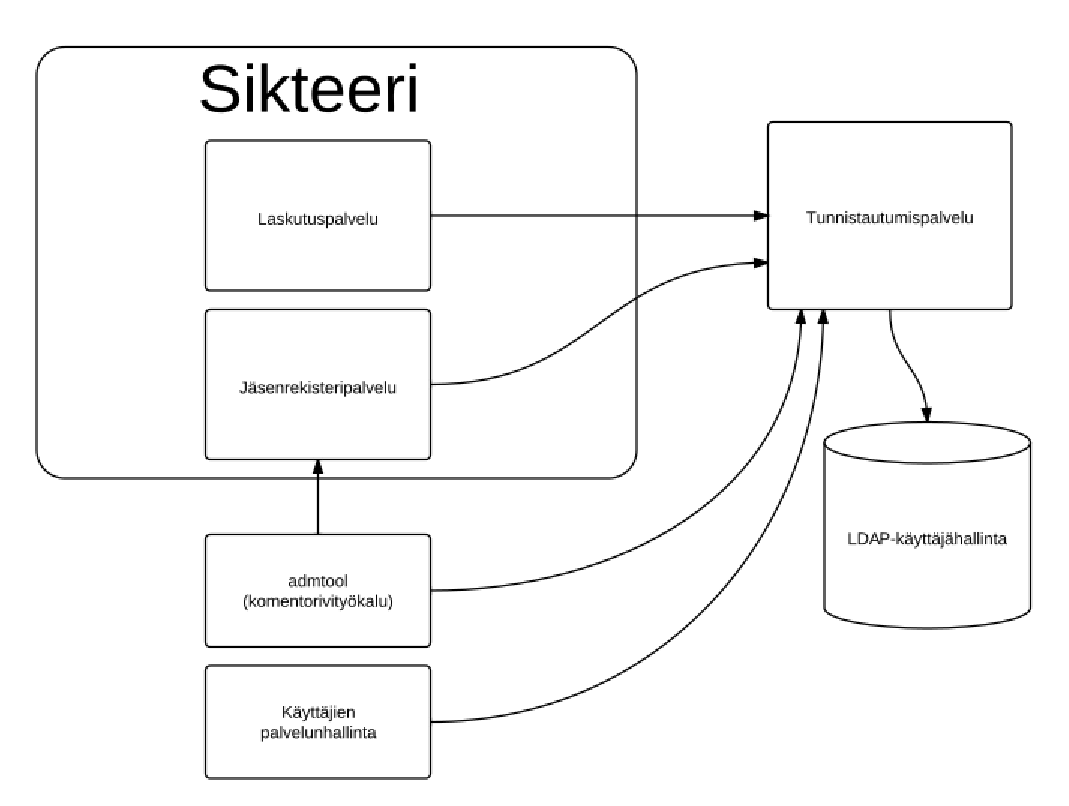
\includegraphics[width=.7\textwidth]{toteutus/kapsi_uusi.eps}
\caption{Keskitettyä tunnistautumispalvelua käyttävä hallintatyökalujen arkkitehtuuri.}%
\label{kapsi_nykyinen_uusi}
\end{figure}

Tulevaisuudessa myös nykyinen Sikteeri halutaan jakaa pienempiin osapalveluihin palvelusuuntautuneiden arkkitehtuurien mukaisesti.Kuvassa \ref{kapsi_uusi} on esitetty tavoiteltu arkkitehtuuri, jossa Sikteerin laskutus- ja jäsenrekisteripalvelut ovat itsenäisiä web-sovelluksia ja joiden rinnalla on admtool-komentorivityökalu sekä käyttäjien palvelunhallinta.

\begin{figure}[ht]
\centering
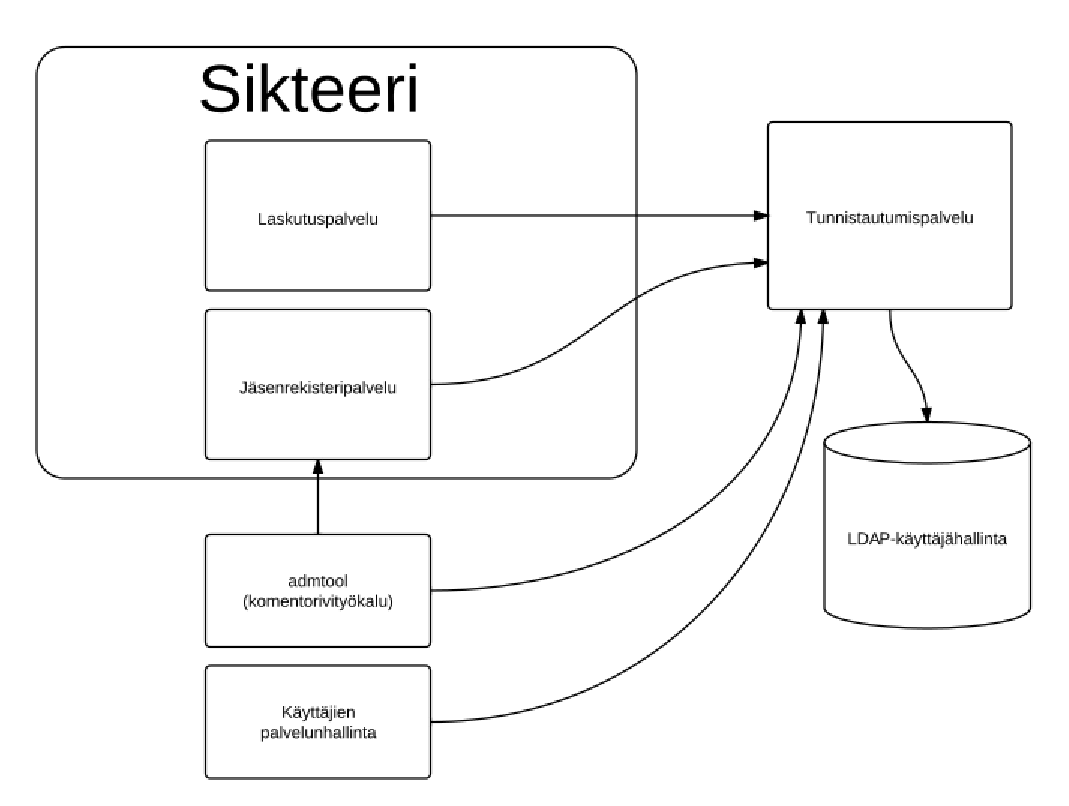
\includegraphics[width=.7\textwidth]{toteutus/kapsi_uusi.eps}
\caption{Palvelusuuntautuneen arkkitehtuurin mukainen kuvaus Kapsin järjestelmästä. Sikteerin palvelut on jaoteltu omiksi komponenteiksi ja järjestelmään on lisätty keskitetty tunnistautumispalvelu.}%
\label{kapsi_uusi}
\end{figure}